\documentclass[../Elmag-labhefte-2020.tex]{subfiles}


\begin{document}

\chapter{ELEKTROSTATISK KRAFT \label{ch.coulomb}}

\subsection*{Mål}

Du skal i denne laboratorieoppgaven
%
\begin{itemize}
\item gjenta Coulombs epokegjørende eksperiment fra 1785, dvs.\ måle elektrostatisk kraft sfa.\ avstand,
\item studere den elektrostatiske kraftens avhengighet av ladningen,
\item bestemme den elektriske permittiviteten for luft,
\item føre en grundig journal og foreta en grundig feilanalyse.
\end{itemize}
%


%**********************************************
\section{Teoretisk bakgrunn}
%**********************************************

Her presenteres teorien svært kort. Noe teori gjennomgås også i teksten til beregningsoppgavene i avsnitt \ref{ch.coulomb.beregn}. Ellers vises til lærebok og forelesningene i elektrisitet og magnetisme.

%**********************************************
\subsection{Coulombs lov}
%**********************************************

Den elektrostatiske kraften (Coulombkraften) $F_\text{e}$ mellom to punktladninger $q_1$ og $q_2$ i en avstand $r$ i tomt rom  er gitt av Coulombs lov:
\begin{equation}
    F_\text{e}
        = \frac{1}{4\pi\epsilon_0} \frac{q_1 q_2}{r^2}
    \label{eq:coulomb}
\end{equation}
hvor $\epsilon_0 = \SI{8,854e-12}{\farad/\m}$ er tomromspermittiviteten. 

%**********************************************
\subsection{Kraftsensoren}
\label{subsec.kraftsensor}
%**********************************************

Coulomb brukte i sitt eksperiment i 1785 ei torsjonsvekt\footnote{Ei torsjonsvekts virkemåte ble grundig gjennomgått i eksperimentet for bestemmelse av gravitasjonskonstanten i labbkurset i Mekanisk fysikk, og vi henviser derfor til labbheftet i Mekanisk fysikk for en detaljert beskrivelse og virkemåte.} for å måle den elektrostatiske kraften mellom to ladde metallkuler og dermed etablere invers kvadrat-forholdet mellom kraft og avstand. Det er alminnelig å representere avvik fra invers kvadrat-loven ved å uttrykke avstandsavhengigheten som $r^{-2\pm q}$. Coulombs verdi for $q$ er \num{4e-2}. Det har vært mange forsøk på å finne en mer presis verdi. I 1971 undersøkte Williams, Faller og Hill\footnote{\textit{Phys. Rev. Lett.} \textbf{26}, 721 (1971)} gyldigheten av Coulombs lov i det hittil mest nøyaktige  ``makroskopiske'' eksperiment som har vært gjennomført. Gitt avstandsavhengighet på formen $r^{-(2+q)}$, fant de at $q = \num{2,7\pm3,1e-16}$.

I eksperimentet skal du bruke en kraftsensor for å gjenta Coulombs eksperiment. Siden kraftsensoren gir en direkte måleverdi, er det viktig for oss å ha en av forståelse hvordan denne virker, og hvorfor den oppgir de måltall den gjør.


%******************************************
\subsubsection{Strekklapp}\vspace{-5mm}
%******************************************
Den ohmske motstanden til et materiale med lengde $l$ og et tverrsnittareal $A$ er gitt ved   
\begin{equation}
    R = \rho \frac{l}{A},
    \label{eq:R_sfa_lA}
\end{equation}
der $\rho$ er spesifikk motstand for materialet. Dette kan utnyttes til å lage en strekksensor, som øker motstanden dersom lengden på en leder økes og reduserer motstanden tilsvarende dersom lederen blir komprimert. Tversnittarealet avtar også noe ved forlengelse og øker noe ved komprimering. Dette vil, sett ut i fra ligning \eqref{eq:R_sfa_lA}, være en fordel da vi ønsker størst mulig målbar endring i motstanden.

En strekklapp (strain gauge sensor) er en leder lagt på en elastisk folie på en slik måte at en endring i en dimensjon lett kan registreres, mens en endring i de andre dimensjonene ikke påvirker sensoren betydelig. En typisk strekklapp er vist i figur \ref{fig:strekklapp}. Hvilken retning er den sensitive retning for målinger og hvorfor?

\begin{figure}[h!b]
    \centering
    \includegraphics[width=6.01cm,height=3cm,keepaspectratio]{fig/strekklapp.png}
    \caption{%
        En strekklapp er en leder (i svart) lagt på en elastisk folie, her vist i forstørret utgave. Pilene er kun som hjelpemiddel for å plassere strekklappen riktig. De store områdene i enden av lederen er loddepunkter for tilkopling av ledning.
    }   
    \label{fig:strekklapp}
\end{figure}


%******************************************
\subsubsection{Wheatstones bro}\vspace{-5mm}
%******************************************
Wheatstones bro, som i bunn og grunn består av to spenningsdelere\footnote{Se kapittel \ref{lorentz.spenningsdeler} for en repetisjon/innføring av hva en spenningsdeler er.}, er en klassisk og effektiv måte å kunne finne verdien av en ukjente motstander. Broen består av en kjent spenningskilde, fire motstander, og et følsomt måleinstrument (galvanometer eller multimeter). Tradisjonelt ble et slik oppsett brukt til å måle størrelsen på en ukjent motstand ved å la den inngå i broen sammen med en kjent motstand og med en nøyaktig variabel motstand (skyvemotstand) koplet inn for den ene spenningsdeleren. 
I figur \ref{fig:wheatstonebridge} ville typisk $R_1$ og $R_2$ være skyvemotstanden, $R_3$ ha kjent verdi, og $R_4$ være den ukjente motstanden. Man stiller inn skyvemotstanden og finner når måleinstrumentet ikke viser noe utslag.  Forholdet mellom den kjente og ukjente motstanden er da gitt av forholdet på skyvemotstanden, og man kan da regne ut verdien av den ukjente motstanden. 


\begin{figure}[htbp]
    \centering
    \includegraphics[height=3cm,keepaspectratio]{wheatstonebridge.eps}
    \caption{%
        Klassisk oppstilling av en Wheatstone-bro, med spenningskilde $V_\text{inn}$, fire motstander $R_1$ -- $R_4$, og et målepunkt $V_\text{ut}$.
    }
    \label{fig:wheatstonebridge}
\end{figure}


%******************************************
\subsubsection{Kraftsensoren} \vspace{-5mm}
%******************************************
I selve kraftsensoren benyttes Wheatstone-broen litt annerledes enn forklart ovenfor. Istedet for å variere motstandene til utspenningen $V_\text{ut} = 0$, leses bare spenningen av som et mål på hvor forskjellige motstandene er. Det benyttes fire strekklapper på et tilpasset legeme, plassert slik at to komprimeres og to strekkes. Figur \ref{fig:ForceSensor} viser et tverrsnitt av kraftsensoren som vi benytter i vårt eksperiment. De fire strekklappene er identiske når sensoren ikke har belastning og har en verdi på $R$, når de utsettes for en belastning (enten strekk eller komprimering) betegner vi endringen ${\Delta R}$. 

Ut i fra likning \eqref{eq:R_sfa_lA} ser vi at en endring i motstand i en strekklapp er proporsjonal med endring i dennes lengde\footnote{Tversnittet av lederen i strekklappen endrer seg ikke i betydelig grad.}. Videre kan vi anta at Hookes lov gjelder for materialet i sensoren, altså at en endring i lengde er proporsjonal med påtrykt kraft. Dette medfører at endringen i motstanden $\Delta R$ er proporsjonal med kraften. Det kan vises at utgangsspenningen, $V_\text{ut}$, er proporsjonal med endringen i motstand, $\Delta R$, og dermed ser vi at utgangsspenningen til kraftsensoren er lineært avhengig av kraften den skal måle\footnote{Sammenhengen mellom utspenning, $V_\text{ut}$,  og endring i motstand, $\Delta R$, er gitt i ligning \eqref{eq:fullbridge}. Denne sammenhengen skal dere selv komme frem til i en av forhåndsoppgavene i kapittel \ref{ch.coulomb.beregn}.}. 

Kraftsensoren koples til en ``universal visningsenhet'' som regner om utsignalet til kraft målt i \si{\milli\newton}.  Denne omregningen, kalibreringen, kan vi ikke endre men den bør etterprøves. Enheten har en nullstillingsknapp markert $\rightarrow 0 \leftarrow$, ved å trykke på denne benytter enheten seg av nåværende verdi av utspenningen, $V_\text{ut}$, som nullreferansepunkt for videre beregning av kraft. Kraftsensoren og visningsenhetens elektronikk krever en viss oppvarmingstid før denne stabiliserer seg. Sørg derfor å skru på enheten minst en halv time før de reelle måleseriene tas for å unngå drift. Det samlede oppsettet for forsøket er vist i figur \ref{fig:CoulombSetUp_new}.

\begin{figure}[!htbp]
    \centering
    \includegraphics[width=12cm,height=8cm,keepaspectratio]{ForceSensor.png}
    \caption{%
        Tverrsnitt av kraftsensoren som består av et metallstykke med som bøyes i enkelte punkter. Fire strekklapper med lik motstand $R$ er plassert i de punkter hvor metallet har størst påkjenning og resistansen i disse endres med $\Delta R$ ved belastning.
    }
    \label{fig:ForceSensor}
\end{figure}

\begin{figure}[h!t]
    \centering
    \includegraphics[width=15cm,height=7.5cm,keepaspectratio]{CoulombSetup-new.png}
    \vspace{-2mm}
    \caption{%
        Forsøksoppstillingen i Coulombeksperimentet. 
	        (1) visningsenheten, 
	        (2) kraftsensor med arm og kondensatorkule K\textsubscript{2}, 
	        (3) målestativ med kondensatorkule K\textsubscript{1}, 
	        (4) ladningsøsen med kondensatorkule K\textsubscript{3}, og
	        (5) høyspenningskanonen.
        Faradayburet er ikke vist.
     }
   \label{fig:CoulombSetUp_new}
\end{figure}

\clearpage


%%%%%%%%%%%%%%%%%%%%%%%%%%%%%%%%%%%%%%%%%%%%%%%%%%%
\section{Beregningsoppgaver/forhåndsoppgaver \label{ch.coulomb.beregn}}
%%%%%%%%%%%%%%%%%%%%%%%%%%%%%
\subsection{Wheatstone-broen}
Oppsettet som kraftsensoren bruker for å måle endring i motstand kalles en full-bro (full bridge), denne skal vi se litt nærmere på.

{\itsf 1. Ut fra figur \ref{fig:wheatstonebridge} og \ref{fig:ForceSensor}, vis at sammenhengen mellom innspenningen $V_\text{inn}$ og utspenningen $V_\text{ut}$ er gitt ved formelen }
\begin{equation}
    \label{eq:fullbridge}
    V_\text{ut} = \frac{\Delta R}  {R} V_\text{inn} .
\end{equation}

Tips: Siden et voltmeter har en stor indre motstand, kan du anta at strømmen gjennom utgangen er null.\\
En typisk hvilemotstand (motstanden uten belastning) for en strekklapp er \SI{120}{\ohm}.


\subsection{Metallkule i tomt rom}

En elektrodes evne til å ta opp ladning avhenger bl.a. av elektrodens kapasitans definert ved
\begin{equation}
    C = \frac{q}{V},
    \label{eq:coulomb.3.1}
\end{equation}
der $q$ er elektrodens ladning og $V$ elektrodens potensial (spenning) relativt uendelig. For ei metall\-kule med radius $\rho$ kan vi fra Gauss' lov beregne at kapasitansen i tomt rom er
\begin{equation}
    C = 4\pi\, \epsilon_0 \, \rho .
    \label{eq:coulomb.3.2}
\end{equation}
%
I eksperimentet skal du anvende kuleformede elektroder med radius $\rho = \SI{15}{\milli\m}$.

{\itsf 2A.  Beregn kapasitansen til en slik elektrode.}
%Svar: 1,67 pF.

{\itsf 2B.  Beregn ladningen på elektroden når den er ladet opp til et elektrisk potensial lik \SI{25}{\kilo\volt}. }
% 20 nC.

\subsection{Bestemmelse av ladning vha. Faradaybur \label{ch.Faradaybur}}
%%%%%%%%%%%%%%%%%%%%%%%%%%%%%

Ifølge Coulombs lov \eqref{eq:coulomb} er det en frastøtende kraft mellom like elektriske ladninger. Ladninger på en elektrode vil derfor søke seg lengst mulig vekk fra hverandre og følgelig fordele seg jamt over elektrodens ytre overflate. Inne i elektroden vil det da være både ladningfritt og feltfritt. Dette ble bevist av Faraday.
\begin{figure}[!ht]
    \centering
    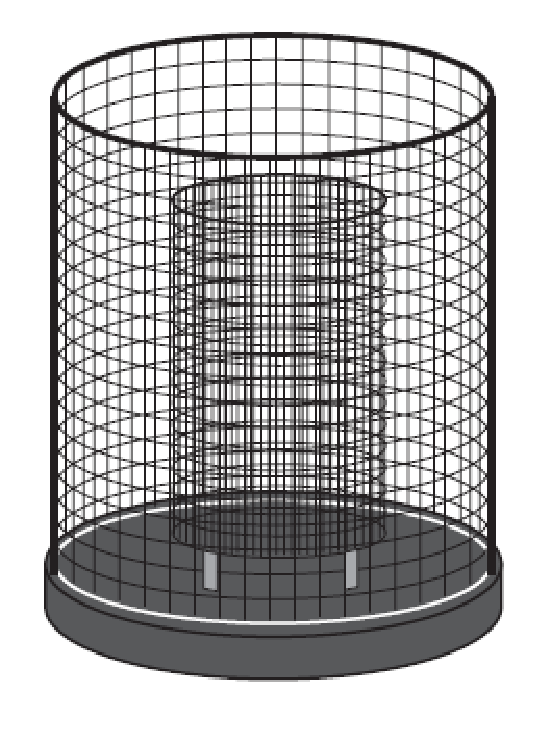
\includegraphics[scale=0.5]{FaradayBur.eps}
    \vspace{-5mm}
    \caption{%
        Faradayburet.
    }
    \label{fig:FaradayBur}
    \vspace{-5mm}
\end{figure}
 
\begin{figure}[!ht]
    \vspace{-2cm}
    \hspace{2cm}
    \setlength{\unitlength}{1mm}
    \begin{picture}(40, 60)(-70,20)       
        \thicklines
        \put(25, 45){\Large\sf C}
        \put(35, 39.5){\circle{6}}
        \put(37, 41.8){\line(1, 1){9.8}}
        \put(37.4, 40.7){\line(1, 1){10}}
        \put(40, 20){\oval(20,10)[b]}
        \put(30, 20){\line(0, 1){25}}
        \put(50, 20){\line(0, 1){25}}
        \put(30, -5){\framebox(20,10)}
        \put(30, 7){\small\sf elektrometer}
        \put(40, 1.75){\oval(16,4)}
        \put(33.5, 0.7){\small\sf 0123456}
        \color{red}
        \put(36, -2.5){\circle{2}}
        \put(36, -2.5){\circle{3}}
        \qbezier(31, 17)(1, 3)(36, -2.5)
        \color{magenta}
        \put(37, 45){\vector(1, 1){9.8}}
        \color{blue}
        \put(44, -2.5){\circle{2}}
        \put(44, -2.5){\circle{3}}
        \put(44, -2.5){\line(0, -1){6}}
        \put(41, -9){\line(1, 0){6}}
        \put(42, -10){\line(1, 0){4}}
        \put(43, -11){\line(1, 0){2}}
        \color{red}
        \put(26, 30){\large$+$}
        \put(26, 35){\large$+$}
        \put(26, 25){\large$+$}
        \put(35, 12){\large$+$}
        \put(41, 12){\large$+$}
        \put(26, 20){\large$+$}
        \put(51, 30){\large$+$}
        \put(51, 35){\large$+$}
        \put(51, 25){\large$+$}
        \put(51, 20){\large$+$}
    \end{picture}
    \begin{picture}(40, 60)(20,20)
        \thicklines
        \put(25, 45){\Large\sf B}
        \put(33, 39.5){\circle{6}}
        \put(35, 41.8){\line(1, 1){9.8}}
        \put(35.4, 40.7){\line(1, 1){10}}
        \put(40, 20){\oval(20,10)[b]}
        \put(30, 20){\line(0, 1){25}}
        \put(50, 20){\line(0, 1){25}}
        \put(30, -5){\framebox(20,10)}
        \put(30, 7){\small\sf elektrometer}
        \put(40, 1.75){\oval(16,4)}
        \put(33.5, 0.7){\small\sf 0123456}
        \color{blue}
        \put(44, -2.5){\circle{2}}
        \put(44, -2.5){\circle{3}}
        \put(44, -2.5){\line(0, -1){6}}
        \put(41, -9){\line(1, 0){6}}
        \put(42, -10){\line(1, 0){4}}
        \put(43, -11){\line(1, 0){2}}
        \color{red}
        \qbezier(31, 17)(1, 3)(36, -2.5)
        \put(36, -2.5){\circle{2}}
        \put(36, -2.5){\circle{3}}
        \put(26, 30){\large$+$}
        \put(26, 35){\large$+$}
        \put(26, 25){\large$+$}
        \put(35, 12){\large$+$}
        \put(41, 12){\large$+$}
        \put(26, 20){\large$+$}
        \put(51, 30){\large$+$}
        \put(51, 35){\large$+$}
        \put(51, 25){\large$+$}
        \put(51, 20){\large$+$}
    \end{picture}
    \begin{picture}(40, 60)(110,20) 
        \thicklines
        \put(25, 45){\Large\sf A}
        \put(35, 39.5){\circle{6}}
        \put(37, 41.8){\line(1, 1){9.8}}
        \put(37.4, 40.7){\line(1, 1){10}}
        \color{red}
        \color{black}
        \put(30, 7){\small\sf elektrometer}
        \put(30, -5){\framebox(20,10)}
        \put(40, 20){\oval(20,10)[b]}
        \put(30, 20){\line(0, 1){25}}
        \put(50, 20){\line(0, 1){25}}
        \put(40, 1.75){\oval(16,4)}
        \put(33.5, 0.7){\small\sf 0123456}
        \color{blue}
        \put(44, -2.5){\circle{2}}
        \put(44, -2.5){\circle{3}}
        \put(44, -2.5){\line(0, -1){6}}
        \put(41, -9){\line(1, 0){6}}
        \put(42, -10){\line(1, 0){4}}
        \put(43, -11){\line(1, 0){2}}
        \color{green}
        \put(44, 54){\vector(-1, -1){9.8}}
        \color{red}
        \qbezier(31, 17)(1, 3)(36, -2.5)
        \put(36, -2.5){\circle{2}}
        \put(36, -2.5){\circle{3}}
        \put(33,38.2){\Large$+$}
        \put(33.1,38.3){\Large$+$}
        \put(32.9,38.1){\Large$+$}
        \put(26, 30){\large$+$}
        \put(26, 35){\large$+$}
        \put(26, 25){\large$+$}
        \put(35, 12){\large$+$}
        \put(41, 12){\large$+$}
        \put(26, 20){\large$+$}
        \put(51, 30){\large$+$}
        \put(51, 35){\large$+$}
        \put(51, 25){\large$+$}
        \put(51, 20){\large$+$}
        \color{blue}
        \put(31, 30){\large$-$}
        \put(31, 35){\large$-$}
        \put(31, 25){\large$-$}
        \put(35, 16){\large$-$}
        \put(41, 16){\large$-$}
        \put(31, 20){\large$-$}
        \put(46, 30){\large$-$}
        \put(46, 35){\large$-$}
        \put(46, 25){\large$-$}
        \put(46, 20){\large$-$}
    \end{picture}
    \vspace{3cm}
    \caption{%
        Måling av ladning med Faradaybur og elektrometer. Faradayburet er isolert fra jord og potensialet relativt jord måles. A: Ladd elektrode føres inn i Faradayburet og elektrometeret viser umiddelbart utslag. B: Elektroden i kontakt med Faradayburet. C: Elektroden trekkes ut og elektrometeret viser fortsatt samme utslag. Elektrodens opprinnelige ladning er overført til Faradaybur/ledning/elektrometer.
    }
    \label{fig:FaradayExpt}
\end{figure}
Faraday isolerte ei metallbøtte elektrisk og kopla et elektroskop til utsiden av bøtta. Så senka han ei ladd metallkule, der kula var festa i en silketråd (som er en god isolator), ned i bøtta. Idet kula kom i kontakt med bunnen viste elektroskopet at bøtta endret tilstand fra uladd til ladd. Elektroskopet viste også utslag før kula var i fysisk kontakt med bøtta, og da kula ble tatt opp av bøtta viste undersøkelser at den var uladd. Dette tolket Faraday slik at når kula berører bunnen av bøtta og blir en del av denne, elektrisk sett, så vil ladningene (som opprinnelig satt på kulas utside) flytte seg til utsida av bøtta.

Vi kan bruke Faradays oppstilling for å måle ladningen på en oppladd elektrode: Faradayburet er vist i figur \ref{fig:FaradayBur} og oppstillingen er vist i figur \ref{fig:FaradayExpt}.  Elektroden med ladningen som skal måles, senkes ned i den innhule elektroden, det såkalte Faradayburet, som er godt isolert fra jord og tilsvarer bøtta i Faradays eksperiment. I stedet for et elektroskop bruker vi et elektrometer for å måle spenningen $V_\text{f}$ på Faradayburet i forhold til jord.  


Faradayburet, ledningene til elektrometeret og selve elektrometeret kan betraktes som en elektrodekonfigurasjon som har en bestemt konstant kapasitans $C = C_\text{Faradaybur} + C_{\rm ledninger} + C_\text{elektrometer}$ mot jord.  Hvis denne kapasitansen er kjent (eller den kan måles), kan ladningen beregnes fra $q = C V_\text{f}$.

Anta at $C = \SI{130}{\pico\farad}$ og at en spenningen $V_\text{f} = \SI{60}{\volt}$ blir målt når en bestemt ladet elektrode senkes ned i Faradayburet.

{\itsf 3.  Beregn ladningen $q$ på elektroden.}
% Svar: 7,8 nC.

Selve Faradayburet er isolert fra jord, men omgitt av en jordet nettingsylinder som skjermer mot elektromagnetisk støy. En koaksialkabel (se figurene \ref{fig:CoaxCable} og \ref{fig:BNC03}) 

\begin{figure}[!h]
    \begin{minipage}[b]{0.5\linewidth}
        \centering
        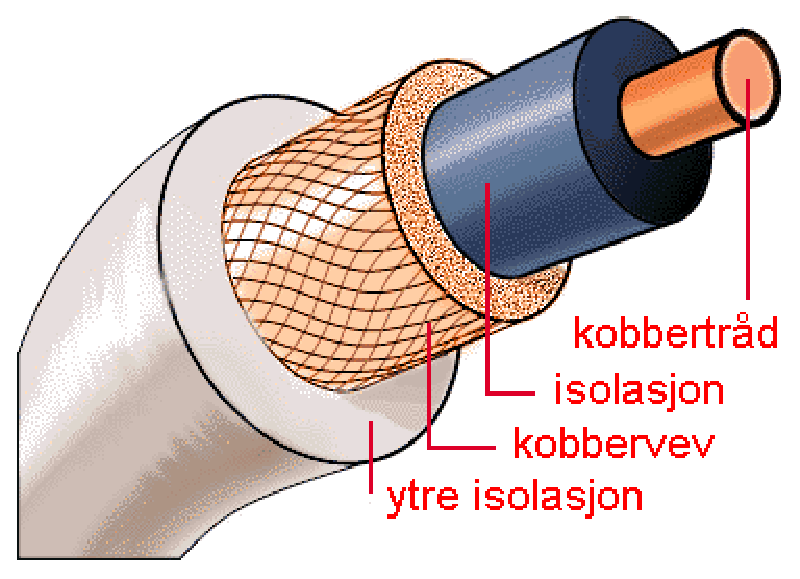
\includegraphics[scale=0.45]{CoaxCable.eps}
        \caption{%
            Tverrsnitt av en koaksialkabel.
        }
        \label{fig:CoaxCable}
    \end{minipage}
    \hspace{0.15cm}
    \begin{minipage}[b]{0.5\linewidth}
        \centering
        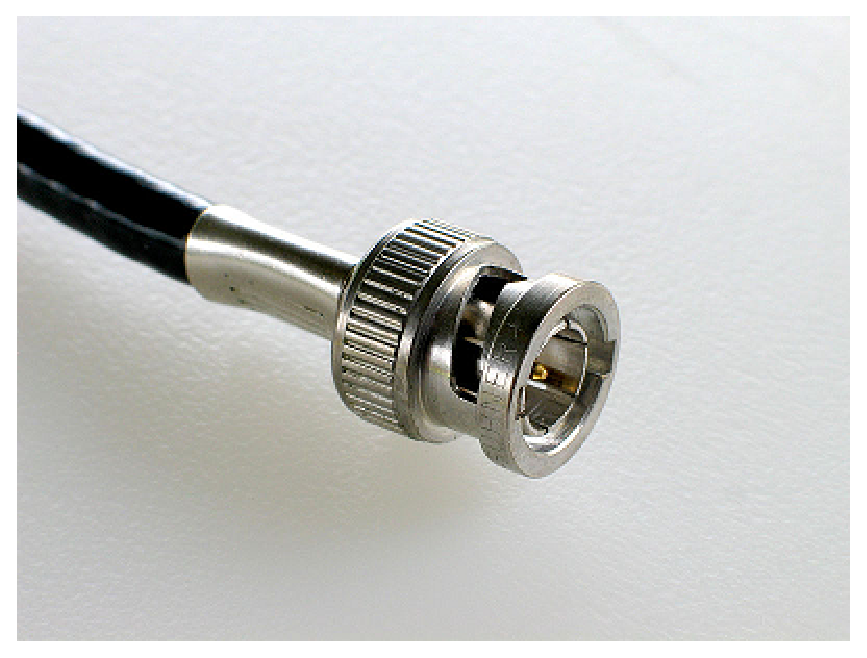
\includegraphics[width=6cm,height=4.5cm,keepaspectratio]{BNC03.eps}
        \caption{%
            Koaksialkabel med BNC-tilkopling.
        }
        \label{fig:BNC03}
    \end{minipage}
\end{figure}
er kopla til elektrometeret. Denne kabelen har to klemmer hvorav senterlederen koples til Faradayburet og skjermledningen til den omgivende nettingsylinderen. Dette er skissert i figur \ref{coulomb.fig1b}. I tillegg koples en jordledning fra elektrometerets jordpunkt til jordingsskjermen. Elektrometeret måler spenningen mellom inngangsklemmene ved at spenningen koples over en kjent, stor motstand $R_\text{i}$ mellom inngangsklemmene, og strømmen $I$ i motstanden måles. Fra Ohms lov beregnes spenningen $V_\text{f} = R_\text{i}  I$, og elektrometerets skala viser spenningen $V_\text{f}$ direkte. 

\begin{figure}[!h]
    \vspace{-1cm}
    \hspace{2cm}
    \setlength{\unitlength}{0.8mm}
    \begin{picture}(40, 60)(-50,20)        
        \thicklines
        \put(40, 20){\oval(20,10)[b]}
        \put(30, 20){\line(0, 1){25}}
        \put(50, 20){\line(0, 1){25}}
        \multiput(15,-4)(0,6){10}{\line(0, 1){5}}
        \multiput(65,-4)(0,6){10}{\line(0, 1){5}}
        \put(31, 0){\oval(16,8)[br]}
        \put(49, 0){\oval(16,8)[bl]}
        \put(39, 0){\line(0, 1){15}}
        \put(41, 0){\line(0, 1){15}}
        \put(-30, -5){\framebox(30,22)}
        \qbezier(-23, 9)(-16, 12)(-9, 9)
        \qbezier(-25, 12)(-16, 15)(-7, 12)
        \qbezier(-25, 12)(-24, 11)(-23, 9)
        \qbezier(-9, 9)(-8, 11)(-7, 12)
        \qbezier(-14, 10.5)(-13, 12)(-12, 13)
        \put(-25, -1){\circle{2}}
        \put(-25, -1){\circle{3}}
        \put(-20, -1){\circle{2}}
        \put(-20, -1){\circle{3}}
        \put(-17.5, -2.5){\small\sf GND}
        \put(25, -10){\sf jordingsplate}
        \put(55, 58){\sf jordingsskjerm}
        \put(38, 48){\sf Faradaybur}
        \put(42, 8){\sf isolerende}
        \put(42, 3){\sf fot}
        \put(-4, 12){\circle{2}}
        \put(-4, 12){\circle{3}}
        \put(-4, 7){\circle{2}}
        \put(-4, 7){\circle{3}}
        \put(-4, 2){\circle{2}}
        \put(-4, 2){\circle{3}}
        \linethickness{0.4mm}
        \qbezier(-20, -1)(-12, -12)(12, -5)
        \linethickness{1.5mm}
        \qbezier(-25, -1)(-55, 16)(-5, 52)
        \linethickness{0.4mm}
        \qbezier(-5, 52)(6, 58)(15, 40)
        \qbezier(-5, 52)(24, 72)(30, 45)
        \put(30, 45){\circle{1.5}}
        \put(15, 40){\circle{1.5}}
        \linethickness{1mm}
        \put(10, -4.5){\line(1, 0){60}}
    \end{picture}
    \vspace{3cm}
    \caption{%
        Faradaybur med omgivende skjerm og elektriske koplinger.
    }
    \label{coulomb.fig1b}
\end{figure}

Ladningen som tilføres elektrometeret for måling vil altså lekke til jord gjennom $R_\text{i}$. Motstanden $R_\text{i}$ må derfor velges stor, ellers vil ladningen forsvinne før du får målt den. Den kan heller ikke velges for stor, da strømmen $I$ blir for liten til å måles nøyaktig.

Anta at $R_\text{i} = \SI{e14}{\ohm}$, $V_\text{f} = \SI{60}{\volt}$ og at $q$ er som beregnet ovenfor.

{\itsf 4. Anslå hvor stor del av ladningen som lekker til jord gjennom elektrometeret i løpet av fem minutter.}
\\
Hjelp: Gjennomfør anslaget ved å anta at $V_\text{f}$ er tilnærmet konstant over fem minutter.

{\itsf 5. Er antakelsen om konstant $V_\text{f}$ rimelig?}
% I = V_f / R = 0,6 pA.  q = It = 180 pC.  (2,3% av 7,8 nC)

\emph{Sikkerhet med elektrometeret:}\\
Elektrometeret kan måle spenninger opp til maksimum \SI{100}{\volt}. Vesentlig høyere spenninger vil skade elektrometeret. Da inngangsmotstanden er så stor som \SI{e14}{\ohm} betyr dette mao. at inngangsstrømmer som er vesentlig større enn $I = V/R = \SI{100}{\volt} / \SI{e14}{\ohm} = \SI{e-12}{\ampere} = \SI{1}{\pico\ampere}$ vil skade elektrometeret.

Kroppen din og klærne lades lett opp til flere tusen volt f.eks. under en rask marsj langs korridoren. Hvis du er oppladet og rører inngangsklemmene til elektrometeret er det en stor sannsynlighet for at du overskrider både strøm- og spenningsbegrensningene til elektrometeret og ødelegger inngangskretsen. Før du begynner å arbeide med elektrometeret er det derfor viktig at du lader ut kroppen din. Dette gjør du \emph{ved å legge begge hender på den jordede skjermplaten som ligger på arbeidsbenken.} Du skal under målingene holde deg utladet ved å la den ene hånda være mest mulig i berøring med skjermplata.

Tilkoplingen til elektrometeret er gjennom en såkalt BNC-kontakt. Denne kontakten er spesielt laget for å brukes sammen med såkalte koaksialkabler. Koaksialkabler er toledere hvor den ene lederen danner en sylindrisk kappe rundt den andre lederen. Den sylindriske kappen brukes som jordleder og skjermer samtidig innerlederen for elektromagnetisk støy. 


Faradayburet består av en \SI{12}{\cm} dyp nettingsylinder med \SI{8}{\cm} diameter, lukket i bunnen og isolert fra fotplata med en \SI{5}{\cm} lang keramikkstav. Ikke berør keramikkstaven med fingrene!  Rundt Faradayburet er det plassert en nettingsylinder som koples til jord for å skjerme Faradayburet mot elektromagnetisk støy. 

\emph{Fremgangsmåte for måling av ladning (se også avsnitt \ref{ch.Faradaybur}): }
\vspace{-4mm}
\begin{itemize}
    \item Sjekk at skjermplata er jordet og rør plata med begge hendene for å utlade deg selv. Sørg deretter for å holde den ene hånda mest mulig på skjermplata. 
    \item Nullstilling av  elektrometeret:
    \vspace{-2mm}
    \begin{itemize}
        \item La elektrometeret være avslått med ZERO-knappen i stilling "ZERO LOCK". Da er inngangen på elektrometeret lagt til GND-kontakten på elektrometeret.
        \item Sett funksjonsknappen på \SI{100}{\volt} og slå elektrometeret på.
        \item  Juster nullpunktet med ZERO-ADJUST-knappen, først med funksjonsvelgeren i stilling \SI{100}{\volt}, deretter med funksjonsvelgeren i stilling \SI{10}{\volt}.  \\
        MERK: Elektrometerets viserinstrument viser korrekt verdi kun når det ligger i horisontalt, reis derfor ikke opp instrumentet. 
        \item Sett funksjonsvelgeren i stilling \SI{100}{\volt}. 
        \item Slå ZERO-knappen over i stilling "PUSH TO ZERO.  Ved å trykke inn ZERO-knappen blir Faradayburet utladet mot jordpotensialet.
    \end{itemize}

\subsection{Coulombs lov \label{ch.coulomb.beregn.coulomb}}
%%%%%%%%%%%%%%%%%%%%%%%%%%

Anta at du har to kuler med radius $\rho = \SI{15}{\milli\m}$, senter-til-senter-avstand \SI{10}{\cm} og at du legger begge på et elektrisk potensial lik \SI{25}{\kilo\volt} relativt uendelig. 

{\itsf 6. Hvor stor blir den elektrostatiske kraften mellom kulene? Blir det tiltrekning eller frastøtning?}

%I 7A og 7B: Regn ut verdier for $F_\text{e}$ i området $3\;{\rm cm} \leq r \leq 15\; {\rm cm}$.

{\itsf 7A. Skisser et kurvediagram over kraften $F_\text{e}$. avhengig av avstand mellom kulene.} Prøv forskjellige valg for x-aksen (for eksempel linear eller kvadratisk).
%Hjelp: Kurva er lineær og og går gjennom origo.

{\itsf 7B. Finn ti verdier for $r$ som vil v\ae re jevnlig fordelt mot $1/r^2$\/} ($\SI{3}{\cm} \leq r \leq \SI{15}{\cm}$)

%{\itsf 7B. Marker en $r$-akse parallelt med $1/r^2$-aksen i diagrammet -- og vis $r$-verdiene som tilsvarer de valgte skalastrekene på $1/r^2$-aksen.}
%\\ Hjelp: $r$-aksens skalainndeling blir selvfølgelig ikke-lineær.

Strengt tatt gjelder Coulombs lov kun for punktladninger. For kuler med endelig utstrekning vil vekselvirkning mellom overflateladningene på kulene gi ujevn ladningsfordeling på kuleoverflatene. Dette vil for to kuler med radius $\rho = \SI{15}{\milli\m}$ i en avstand større enn 10 cm føre til et avvik på under \SI{1}{\percent} i forhold til verdier beregnet vha. Coulombs lov \eqref{eq:coulomb}.Hvor stort feil fører dette til i målingene? 


\subsection{Gravitasjonskraft}

Vi ønsker å måle den elektrostatiske kraften mellom kulene med en så stor nøyaktighet som mulig. I oppsettet vil vi ha gravitasjonsvekselvirkning mellom kulene i tillegg til den elektrostatiske kraften. Kulene veier omtrent \SI{25}{\g} hver. Er gravitasjonskreftene relevant for målingene deres?

%{\itsf 8. Beregn gravitasjonskraften mellom kulene. Er det nødvendig å ta hensyn til gravitasjonskraften mellom kulene?}
% 4,2 pN => << 7,8 nC
 
\clearpage


%%%%%%%%%%%%%%%%%%%%%%%%%%%%%%%%%%%%%%%%%%%%%%%%%%
\section{Eksperimentelt}
%%%%%%%%%%%%%%%%%%%%%%%%%%%%%%%%%%%%%%%%%%%%%%%%%%

%%%%%%%%%%%%%%%%%%%%%%%%%%%%%%%%%%%%%%%%%%%%%%%%%%
\subsection{Apparatur}
%%%%%%%%%%%%%%%%%%%%%%%%%%%%%%%%%%%%%%%%%%%%%%%%%%

Følgende instrumenter inngår i oppstillingen:
\vspace{-4mm} 
\begin{itemize}
    \item \textbf{Kraftsensor} Leybold S  524 060. Measuring error: $< 1\%$
Resolution: $< 0.01 mN$ 
    m/tilbehør:
    \vspace{-2mm} 
    \begin{itemize}
        \item \textbf{Visningsenhet}, Leybold UMI 531 835.
        \item \textbf{Arm med kule}, kulediameter \SI{30}{\milli\m}.
        \item \textbf{kalibreringslodd}, lodd med nøye oppmålte masser.
    \end{itemize}
    \item \textbf{Høyspenningskanon} Emco DX250. Utgangsspenning/strøm: \SI{25}{\kilo\volt}/\SI{75}{\micro\ampere}. Inngangsspenning: +\SI{12}{\volt} $\pm \SI{5}{\percent}$.
    \item \textbf{Spenningskilde}  EA-PS 2012-05 for høyspenningskanon, spenning: \SI{12}{\volt}.
    \item \textbf{Ladningsøse}, kulediameter \SI{30}{\milli\m}.
    \item \textbf{Målestativ med kule}, kulediameter \SI{30}{\milli\m}.
    \item \textbf{Diverse utstyr.} Målestav \SI{1}{\m}; metermål 0-2 \si{\m}; skyvelære; vaterpass; vater m/tvinge, plasthansker.
    \item \textbf{Faradaybur, elektrometer og tilhørende utstyr:}
    \vspace{-2mm}
    \begin{itemize}
        \item \textbf{Skjermet Faradaybur}, Pasco Mod. ES9058.
        \item \textbf{Elektrometer} m/tilkoplingskabler. \\
              Måleområde: 0-\SI{100}{\volt}, inngangsmotstand: $R_\text{i} = \SI{e14}{\ohm}$. 
        \item Faradaybur, kabel og elektrometer har en total kapasitans på $C = \SI{130}{\pico\farad}$. 
        \item \textbf{Multimeter} Escort EDM168A, 3 sifre, eller tilsvarende. 
    \end{itemize}
\end{itemize}

%%%%%%%%%%%%%%%%%%%%%%%%%%%%%%%%%%%%%%%%%%%%%%%%%%
\subsection{Forsiktighetsregler}
%%%%%%%%%%%%%%%%%%%%%%%%%%%%%%%%%%%%%%%%%%%%%%%%%%

\textbf{Høy spenning.}\\
Høyspenningskanonen som brukes for å lade opp kulene gir \SI{25}{\kilo\volt} når den aktiveres. Strømmen er imidlertid begrenset til \SI{75}{\micro\ampere}. Slike strømmer har vanligvis ingen fysiologisk virkning på kroppen, men likevel: \emph{Behandle kanonen som om den var livsfarlig.}

\textbf{Kraftsensoren.}\\
Kraftsensoren er et presisjonsinstrument som du må behandle forsiktig. Dette gjelder spesielt ved å ikke utsette den for krefter større enn $\pm \SI{2,5}{\newton}$, noe som kan føre til overbelasting av sensoren. Sensoren er ikke ment for måling av krefter større enn $\pm \SI{1}{\newton}$. 


\textbf{Isolatorer.}\\
Overflaten av isolatorene som kulene er montert på bør ikke røres med fingrene. Fett og syre fra fingeravtrykk vil danne ledende kanaler på overflaten og nedsette isolasjonsevnen og føre til lekkasje av ladning fra kulene. Bruk utlagte plasthansker når du må håndtere kulene eller isolatorene. 


%%%%%%%%%%%%%%%%%%%%%%%%%%%%%%%%%%%%%%%%%%%%%%%%%%
\subsection{Kalibrering: Etterprøving av kraftsensoren.}
%%%%%%%%%%%%%%%%%%%%%%%%%%%%%%%%%%%%%%%%%%%%%%%%%%

Kraftsensoren er allerede ferdig kalibrert fra Leybold GmbH. Vi vet ikke om det den viser stemmer, og dette bør etterprøves. 
Sett opp kraftsensoren slik at denne kan måle i vertikal retning, sørg for at denne er i lodd, og at sensoren er nullstilt.
 
Foreta målinger med forskjellige masser og fremstill dette i en graf, kraft som funksjon av masse. Estimer stigningstall og en usikkerhet for denne grafen.


%%%%%%%%%%%%%%%%%%%%%%%%%%%%%%%%%%%%%%%%%%%%%%%%%%
\subsection{Montering av kuleelektrode og klargjøring av kraftsensor}
% og dempningsror}
%%%%%%%%%%%%%%%%%%%%%%%%%%%%%%%%%%%%%%%%%%%%%%%%%%

Kraftsensoren må vatres slik at den virker i horisontal retning for de påfølgende eksperimenter. Videre må kulen K\textsubscript{2} monteres på kulearmen og kraftsensoren må nullstilles. En sjekk av nullstilling bør gjøres ofte.

Bruk alltid plasthansker når du må ta på kulene eller kulearmene.


%%%%%%%%%%%%%%%%%%%%%%%%%%%%%%%%%%%%%%%%%%%%%%%%%%
\subsection{Elektriske ledninger}
%%%%%%%%%%%%%%%%%%%%%%%%%%%%%%%%%%%%%%%%%%%%%%%%%%
Prøv alltid å bruke riktig fargekoding på de forskjellige ledningene når du setter opp et eksperiment, dette gjør feilsøking mye enklere. 

\subsubsection{Oppkopling av elektriske ledninger:}

\vspace{-4mm}
\begin{itemize}
    \item Kople høyspenningskanonen til spenningsforsyningen: Ledning med rød plugg til +\SI{12}{\volt}, blå med svart endeplugg til \SI{0}{\volt}, gul til jordkontakten.
    \item \SI{0}{\volt} på spenningsforsyningen skal være jordet referanse, kople derfor sammen jordkontakten og \SI{0}{\volt}-uttaket på denne. 
    \item Kople jordledninger til kraftsensorstativet med kule K\textsubscript{2}, målestativet med kule K\textsubscript{1}, ladningsøsen med kule K\textsubscript{3}. 
\end{itemize}

Apparaturen er nå klar til bruk.  Be labveilederen om å demonstrere bruken av kanonen før du tar den i bruk.



%%%%%%%%%%%%%%%%%%%%%%%%%%%%%%%%%%%%%%%%%%%%%%%%%%
\subsection{Eksperiment 1: Kraft sfa. avstand}
%%%%%%%%%%%%%%%%%%%%%%%%%%%%%%%%%%%%%%%%%%%%%%%%%%
 
Oppgave:\\
{\itsf Undersøk hvordan den elektrostatiske kraften mellom de ladde metallkulene K\textsubscript{1} og K\textsubscript{2} varierer som funksjon av senter-til-senter-avstanden $r$. 
}

Kule K\textsubscript{2} er montert på kraftsensoren og kule K\textsubscript{1} er montert på en skyvbar arm slik at avstanden mellom kulene kan reguleres. 


\subsubsection{Analyse av måleresultatene.}
\vspace{-4mm} 
\begin{itemize}
    \item Tegn opp ei kurve av kraften $F_\text{e}$ sfa. $1/r^2$ på millimeterpapir eller i Excel/Python. Estimer en trendlinje.
    \item Beregn gjennomsnitt og standardavvik for hver målte $r$-verdi ut fra de forskjellige måleseriene.
    \item Stemmer resultatene dine med Coulombs lov? Kan du forklare eventuelle avvik? Hva skjer når $r$ er mindre enn 5-\SI{6}{\cm}?
\end{itemize}


Mens du måler vil ladningen gradvis lekke ut fra kulene, spesielt hvis du bruker lang tid på måleserien. Prøv derfor å redusere tiden mest mulig men ivareta nøyaktigheten. Siden forutsetningen er at ladningen på kulene skal være konstant under hver måleserie vil ladningstapet føre til en målefeil. Det er viktig å legge opp måleprosedyren slik at denne feilkilden kan kontrolleres. Du kan derfor  ta \emph{flere måleserier} med utladning og oppladning av kulene mellom hver serie. I første serie måler du (som beskrevet) $F_\text{e}$ for avtakende verdier av $r$ og i neste måleserie måler du $F_\text{e}$ for de samme $r$-verdiene i økende rekkefølge. Sammenlikning av målingene ved tilsvarende avstander mellom de to seriene vil gi opplysninger om forandring av ladningen. En annen måte å kontrollere tap av ladning er å foreta en kontrollmåling ved en bestemt $r$-verdi f. eks. $r = \SI{10}{\cm}$ mellom hver måling. Så lenge resultatet av kontrollmålingen forblir konstant har du ikke mistet ladning. Selv om du oppdager at ladningen begynner å lekke ut kan du fortsette målingen, da systematiske feil er en del av hvor nøyaktig vi kan gjøre disse målingene.

En annen målefeil er at når kule K\textsubscript{2} forskyves som følge av frastøtningen, er ikke avstanden mellom kulene lik det som skalaen indikerer. Dette får mest betydning når kulene er nærme, men denne effekten er nokså liten i vårt eksperiment, da det er snakk om små krefter og kraftsensoren ikke beveger seg langt. Gjør et estimat, om mulig av hvor langt sensoren flytter seg ved full kraft mellom kulene og liten avstand. 

En tredje målefeil skyldes polarisasjon av ladningen på kulene. Like ladninger frastøter hverandre slik at senter-til-senter-avstand for ladningsfordelingen på hver kule er større enn geometrisk senter-til-senter-avstand for kulene. Denne feilen får også mest betydning når kulene er nærme. Gjør et estimat av størrelsen på feilen.

Hva vil skje dersom kulene ikke har like stor ladning?



%%%%%%%%%%%%%%%%%%%%%%%%%%%%%%%%%%%%%%%%%%%%%%%%%%
\subsection{Eksperiment 2: Kraft sfa. ladning }
%%%%%%%%%%%%%%%%%%%%%%%%%%%%%%%%%%%%%%%%%%%%%%%%%%

Oppgave:\\
{\itsf Undersøk hvordan den elektrostatiske kraften avhenger av ladningen $q_1$ til kule K\textsubscript{1}. Dvs. mål Kraften på kule K\textsubscript{2} sfa. ladningen på kule K\textsubscript{1}.} 

Finn en mulighet for å redusere ladningen på kulen på en kontrollert måte og sett opp en måleserie basert på det. Gjenta måleserien flere ganger.

\subsubsection{Analyse av måleresultatene.}

\vspace{-4mm} 
\begin{itemize}
    \item Tegn opp ei kurve av kraften $F_\text{e}$ sfa. ladning $q_1$ på millimeterpapir eller i Excel/Python. Estimer en trendlinje.
    \item Beregn gjennomsnitt og standardavvik for hver $q_1$-verdi.
    \item Stemmer resultatene dine med Coulombs lov? Kan du forklare eventuelle avvik?
\end{itemize}

%http://fcit.usf.edu/network/chap4/chap4.htm
%http://www.google.no/imgres?imgurl=http://www-ece.rice.edu/~jdw/figs/bnc_t.jpg&imgrefurl=http://www.ece.rice.edu/~jdw/unilab.new/file.3.html&h=260&w=327&sz=9&tbnid=4AP2rDHWMwwVdM:&tbnh=94&tbnw=118&prev=/images%3Fq%3DBNC%2Bconnector%2Bsite:.edu&hl=no&usg=__RIEFn0MtcJl4U5WJ9Sm1R_qSZck=&ei=vJ3JSuPLBdPJ-Qby79hH&sa=X&oi=image_result&resnum=4&ct=image

%%%%%%%%%%%%%%%%%%%%%%%%%%%%%%%%%%%%%%%%%%%%%%%%%%
\subsection{Eksperiment 3: Elektrisk permittivitet}
%%%%%%%%%%%%%%%%%%%%%%%%%%%%%%%%%%%%%%%%%%%%%%%%%%

Oppgave:\\
{\itsf Du skal beregne verdi for luftas permittivitet $\epsilon_0$ ved to ulike metoder:

\vspace{-4mm}
\begin{itemize}
    \item[I)] Måling av ladning og kraft på kule og bruk av Coulombs lov \eqref{eq:coulomb}.
    \item[II)] Beregning av kapasistans for kule via ladningsmåling og antakelse om kapasistans for ei kule i likning \eqref{eq:coulomb.3.2}.
\end{itemize}
}

\textbf{\emph{Metode I:}}

I eksperiment 1 har du målt den elektrostatiske kraften $F_\text{e}$ mellom to metallkuler. Hvis du også måler ladningen på kulene, kan du fra Coulombs lov \eqref{eq:coulomb} bestemme luftas permittivitet $\epsilon_0$ når avstanden er kjent. Ladningsmåling kan gjøres ved Faradaybur og elektrometer, som forklart i det følgende, med referanse til avsnitt \ref{ch.Faradaybur}.


%
    \item Bestemmelse av ladningen på kule K\textsubscript{3} (ladningsøsa):
    \vspace{-2mm} 
    \begin{itemize}
        \item Lad kula K\textsubscript{3} med høyspenningskanonen. 
        \item Før kula til kontakt med Faradayburets innside for å måle  spenningen på Faradayburet.
        \item Gjenta målingen flere ganger for å få statistisks avvik.
        \item Test også tidsstabilteten av den målte spenningen. Er spenningen stabilt? Hvis ikke, hva er grunnen og hvordan kan en ta hensyn til det? 
        \item Etter endt måling, sett ZERO-knappen i stilling "ZERO LOCK" og slå av elektrometeret.
        \item Beregn ladningen på kula. Anta at Faradayburet, kabel og elektrometer har total kapasitans $C = \SI{130}{\pico\farad}$.
%Verdien er funnet fra oppgitt inngangskapasitans på $C =$ 30 pf for elektrometeret og målt kapasitans for kabelen, og du kan etterprøve verdien for kabelen vha. multimeteret. 
    \end{itemize}
\end{itemize}

Du observerte kanskje at elektrometeret fikk det endelige utslaget allerede før du berørte gitteret? Dette kalles induksjon og skyldes at ladningen på giveren tiltrekker/frastøter elektronene i gitteret slik at det på utsiden av gitteret samles en ladning som er like stor som ladningen vi vil måle.

Bruk resultatet for en valgfri verdi av $r$ fra eksperiment 1 til å finne kraften mellom to kuler med full oppladning og med kjent avstand. Kulene K\textsubscript{1} og K\textsubscript{2} har samme dimensjon som kula K\textsubscript{3} på ladningsøsa, slik at de forventes å få samme ladning ved oppladning fra elektronkanonen. Husk halveringen av ladningen på K\textsubscript{3} før måling i Faradayburet.

{\itsf Beregn luftas permittivitet $\epsilon_0$ med usikkerhet fra Coulombs lov i likning (\ref{eq:coulomb}).}

\textbf{\emph{Metode II:}}

Når ladningen er målt og potensialet er kjent, kan du beregne kulas kapasitans fra likning \eqref{eq:coulomb.3.1}. Hvis kulas radius, $\rho$, måles, kan du beregne luftas permittivitet fra uttrykket \eqref{eq:coulomb.3.2} for kulas kapasitans.

Anta at høyspenningskanonen lader opp til \SI{25}{\kilo\volt} og bruk at høyspenningskanonen og kula har samme potensial ved ladningsoverføring til å beregne kapasitansen til kula. 

{\itsf Beregn luftas permittivitet $\epsilon_0$ med usikkerhet fra beregnet kapasitans og bruk av likning \eqref{eq:coulomb.3.2}.}

\subsubsection{Diskusjon:}
\begin{itemize}
    \item Sammenlikn verdien av den målte kulekapasitansen med den beregnede verdien i beregningsoppgave 2A.
    \item Diskuter eventuelle avvik mellom målt og beregnet verdi for kapasitansen. 
     \item Sammenlikn din oppnådde verdi for $\epsilon_0$ med tabellverdi.
    \item Hvordan er overensstemmelsen med estimatet for $\epsilon_0$ med de to beregningsmetoder? Hvilken verdi har minst feil? Begrunn svaret ditt.
    \item Er det samsvar mellom målt verdi og tabellverdi for $\epsilon_0$ innenfor de estimerte feilgrenser?
    \item Dersom noe avviker, gi en begrunnelse hvorfor.  
\end{itemize}


%%%%%%%%%%%%%%%%%%%%%%%%%%%%%%%%%%%%%%%%%%%%%%%%%%%
%\subsection{Diskusjon}
%%%%%%%%%%%%%%%%%%%%%%%%%%%%%%%%%%%%%%%%%%%%%%%%%%%
%
%\begin{itemize}
%\item Sammenlikn måleresultatene fra de ulike deler av eksperimentet.
%\item Diskuter eventuelle uoverenstemmelser. 
%\item Diskuter styrkeforholdet mellom elektrostatisk kraft og gravitasjonskraft.
%\item Diskuter mulige anvendelser av de fysiske effekter som er tatt opp til observasjon i eksperimentet.
%\end{itemize}


%%%%%%%%%%%%%%%%%%%%%%%%%%%%%%%%%%%%%%%%%%%%%%%%%%
\subsection{Avslutning}
%%%%%%%%%%%%%%%%%%%%%%%%%%%%%%%%%%%%%%%%%%%%%%%%%%
\emph{La kraftmåleren stå påslått}, kople fra de andre ledningene og forlat plassen i minst like god orden som du fant den.

\end{document}